\documentclass[12pt]{article}
\usepackage{fullpage,graphicx,psfrag,amsmath,amsfonts,verbatim}
\usepackage[small,bf]{caption}
\usepackage{algorithmicx,algpseudocode}
\usepackage{url,algorithm,amsthm}
\input defs.tex
\usepackage{subcaption}
\usepackage{lscape} % for horizontal pages with results
\usepackage{booktabs}
\usepackage{placeins}
\usepackage{verbatim}

\usepackage{hyperref} %%for clickable references!!
\usepackage{amsthm}
\newtheorem{lem}{Lemma}
\usepackage[toc,page]{appendix}
\graphicspath{{../Graphics/}}
%\usepackage[backend=bibtex,firstinits=true,style=alphabetic]{biblatex}

\title{Distributional Robust Kelly Gambling}
\author{Qingyun Sun \and Stephen Boyd}

\date{}

\begin{document}
\maketitle
\begin{abstract}
We consider the distributional robust version of Kelly gambling problem, in which the probability distribution is not known. 
We maximize the worst-case log growth among all possible distributions in a probability set.
This distributional robust problem is convex, but in general it is not always tractable. In this paper, we show that it
can be solved in finite outcomes case, for some useful probability sets, 
as a tractable convex problem.
\end{abstract}
% 
% * <sunqingyun1708@gmail.com> 2018-08-22T00:15:57.712Z:
%
% ^.
\section{Introduction}
\paragraph{Gambling}
We consider a setting where a
gambler repeatedly allocates a fraction of her wealth 
(assumed positive) across $n$ different bets in multiple rounds.
We let $b \in \reals^n$ denote the bet allocation, so 
$b \geq 0$ and $\ones^Tb=1$, where $\ones$ is the vector with all
entries one. We define $n-$ dimensional simplex as $S_n$, then $b\in S_n$.
In each betting round the bettor's
wealth is multiplied by the random factor $r^T b$, where $r \in \reals_+^n$
is the random payoff or total return vector,
drawn IID from a given distribution.
We will assume that $r_n =1$ almost surely, \ie, the last bet
has no risk (of loss or gain).  Thus $b_n$ is the fraction of 
wealth that is held as cash.
The betting allocation $b=e_n$ corresponds to not betting at all.
The log of the wealth is therefore a random walk, with 
increment distribution given by $\log(r^Tb)$.

We consider here the case where one of $K$ events occurs, \ie, $r$ is supported
on only $K$ points.  We let $r_1, \ldots, r_K$ denote the 
return vectors, and $\pi = (\pi_1, \ldots, \pi_K)\in S_K$ the corresponding
probabilities.
We collect the $K$ possible payoff vectors into a 
matrix $R\in \reals^{n\times K}$, with columns $r_1, \ldots, r_K$.
The vector $R^Tb \in \reals^K$ gives the wealth growth factor in
the $K$ possible outcomes.
The mean log growth rate is
\[
G_\pi(b) = \Expect \log (r^Tb) = \pi^T \log (R^Tb),
\]
where the log term applied to the vector elementwise.
This is the mean drift in the log wealth random walk.

\paragraph{Kelly gambling}
In a 1956 classic paper
\cite{kelly1956new},
John Kelly proposed to choose the allocation vector $b$ so as to
maximize the mean log growth rate $G_\pi(b)$,
subject to $b \geq 0$, $\ones^Tb=1$. This method was named Kelly criterion, and there was lots of influential works on this topic since then \cite{maclean2011kelly, thorp1975portfolio, davis2012fractional,maclean2010long, thorp2011understanding, kadane2011partial}.
The log growth $G_\pi(b)$ is a concave function of $b$,
so this is a convex optimization problem \cite{cvxopt,boyd2004convex}.
It can be solved analytically
in simple cases, such as when there are $K=2$ possible outcomes.
It is easily solved in other cases using standard methods and algorithms,
and readily expressed in various domain specific languages for 
convex optimization such as
CVX \cite{cvx}, CVXPY \cite{cvxpy}, Convex.jl \cite{convexjl}, or CVXR \cite{fu2017cvxr}.
We can add additional convex constraints on $b$, which we denote as $b\in B$,
with $B$ a convex set, while preserving convexity.
While Kelly did not consider additional constraints, we still refer
to the problem of maximizing $G_\pi(b)$ subject to 
$b \geq 0$, $\ones^Tb=1$, and $b\in B$ as the Kelly gambling problem.

There have been many papers exploring and extending the Kelly framework;
for example, a drawdown risk constraint, that preserves convexity
(hence, tractability) is described in \cite{busseti2016risk}. The Bayesian version of Kelly optimal betting is  described in \cite{browne1996portfolio}. In \cite{lo2018growth}, the Kelly criteria is generalized to maximize the proportion of wealth relative to the total wealth in the population.
% XXX add others?
 
\paragraph{Distributional robust Kelly gambling}
In this note we study a distributional robust version of Kelly gambling,
in which the probability distribution $\pi$ is not known.  
Rather, it is known that $\pi \in \Pi$, a set of possible distributions.
We define the worst-case log growth (under $\Pi$) as 
\[
G_\Pi (b) = \inf_{\pi \in \Pi} G_\pi(b).
\]
This is evidently a concave function of $b$, since it is an infimum of 
a family of concave functions of $b$, \ie, $G_\pi(b)$ for $\pi \in \Pi$.
The \emph{distributional robust Kelly problem} (DRKP) is to choose $b$ to maximize
$G_\Pi (b)$, subject to $b \in B$, $b\geq 0$, $\ones^Tb=1$.
This is in principle a convex optimization problem, specifically a 
distributional robust problem; but such problems in general need not
be tractable, as demonstrated in \cite{nemirovski2009robust,nemirovski1978,nemirovski1983}
The purpose of this note is to show how the DRKP
can be solved in finite outcomes case, for some useful probability sets $\Pi$, 
as a tractable convex problem.
\paragraph{Related work on distributional robust optimization}
Distributional robust optimization is a well studied topic. 
Previous work to distribution robust optimization 
studied finite-dimensional parametrization for probability set like moments, 
support or directional deviations constraints in \cite{delage2010distributionally,yang2008distributed,burger2012distributed,goh2010distributionally, chen2007robust, mutapcic2009cutting}.
Beyond finite-dimensional parametrization for probability set, people have also studied non-parametric distances for probability measure, like f-divergences(e.g. Kullback-Leibler divergences) \cite{miyato2015distributional,duchi2016statistics,bertsimas2018data,ben2013robust,namkoong2016stochastic} and Wasserstein distances \cite{blanchet2018distributionally,blanchet2016robust,esfahani2017data,shafieezadeh2015distributionally}. 


\section{Probability sets}
\subsection{Polyhedral probability set}
We consider the case when $\Pi$ is given by a finite set of linear 
inequalities and equalities, 
\BEQ\label{pi-desc}
A_0 \pi = d_0, \quad A_1 \pi \leq d_1,
\EEQ
where $A_0 \in \reals^{m_0 \times K}$, $b_0 \in \reals^{m_0}$, 
$A_1 \in \reals^{m_1 \times K}$, $b_1 \in \reals^{m_1}$.
The worst-case log growth rate $G_\Pi(b)$ is given by the optimal value 
of the linear program (LP)
\BEQ \label{e-GPi}
\begin{array}{ll}
\text{minimize}& \pi^T \log (R^T b) \\
\text{subject to} & \ones^T \pi = 1, \quad \pi \geq 0, \\
& A_0 \pi = d_0, \quad A_1 \pi \leq d_1,
\end{array}
\EEQ
with variable $\pi$.

We form a dual of this problem, working with the constraints
$A_0 \pi = d_0$, $A_1 \pi \leq d_1$; we keep
the simplex constraints $\pi \geq 0$, $\ones^T \pi = 1$ 
as an indicator function $I_S(\pi)$ in the objective.
The Lagrangian is 
\[
L(\nu,\lambda, \pi) = 
\pi^T \log (R^T b)+ \nu^T (A_0\pi-d_0) + \lambda^T (A_1\pi-d_1) + I_S(\pi),
\]
where $\lambda \geq 0$.
Minimizing over $\pi$ we obtain the dual function,
\[
g(\nu,\lambda) = \inf_\pi L(\nu,\lambda,\pi) =
\min (\log (R^T b)+ A_0^T \nu +  A_1^T \lambda ) -  d_0^T \mu- d_1^T \lambda,
\]
where the min of a vector is the minimum of its entries.
The associated dual is then
\[
\begin{array}{ll} \mbox{maximize} &
\min (\log (R^T b)+  A_0^T \mu +  A_1^T \lambda) -  d_0^T \mu- d_1^T \lambda  \\
\mbox{subject to} & \lambda \geq 0,
\end{array}
\]
with variables $\mu, \lambda$.
This problem has the same optimal value as~(\ref{e-GPi}), so we have
\[
G_\Pi (b) = \sup_{\nu, \lambda \geq 0} 
\left(
\min (\log (R^T b)+  A_0^T \mu +  A_1^T \lambda) -  d_0^T \mu- d_1^T \lambda
\right).
\]

Using this expression for $G_\Pi(b)$, we can express the DRKP as the optimization
problem
\BEQ\label{e-DRKP}
\begin{array}{ll}
\text{maximize}&  \min (\log (R^T b)+  A_0^T \mu +  A_1^T \lambda) -
 d_0^T \mu- d_1^T \lambda  \\
\text{subject to} & b\in B, \quad \lambda \geq 0,
\end{array}
\EEQ
with variables $b, \mu, \lambda$.
This is a tractable convex optimization problem, readily expressed 
in domain specific languages for convex optimization.

% XXX GOT HERE

In the following, we list several examples of polyhedral probability set,
and provide their CVXPY specifications.

\paragraph{Convex hull of a finite set}
 When $\Pi$ is a polyhedron defined as the convex hull of a finite set of modest size $\Pi = \mathbf{conv}(\pi, \ldots, \pi_s)$. 

Then the minimum over $\pi \in\Pi$ is the same as the minimum over the given vertices, 
$G_{\Pi} (b) = \min_{i}  G_{\pi_i} (b) = \min_{i} \pi_i^T \log (R^T b)$.
Then the problem becomes
\BEQ\label{ e-LDRKP}
\begin{array}{ll}
\text{maximize}&  \min_i   
\pi_i^T \log (R^T b) 
 \\
\text{subject to} & b\in B,
\end{array}
\EEQ
with variables $b$.

\paragraph{Box probability set}
When $\Pi$ is given by the box constraint
$\{ \pi = \pi_0 + \delta, \quad -l\leq \delta\leq l, \quad \ones^T \pi = 1, \quad \pi \geq 0\}.$ 

We can use the LP duality, the problem becomes 
\BEQ
\begin{array}{ll}
\text{maximize}&  \left(\min_i   (\log (R^T b)+  \lambda_{+}-\lambda_{-})_i \right) -  (\pi_0+l)^T \lambda_{+} - (\pi_0-l)^T \lambda_{-} \\
\text{subject to} & b\in B, \quad \lambda_{+} \geq 0,\quad \lambda_{-} \geq 0,
\end{array}
\EEQ
with variables $b, \lambda_{+}, \lambda_{-}$.
Let $\lambda = \lambda_{+}- \lambda_{-}$, then $|\lambda|= \lambda_{+}+ \lambda_{-}$, the problem becomes
\BEQ\label{ e-LDRKP}
\begin{array}{ll}
\text{maximize}&  \left(\min_i   
(\log (R^T b)+  \lambda)_i \right) 
-  \pi_0^T |\lambda| - l^T \lambda \\
\text{subject to} & b\in B,
\end{array}
\EEQ
with variables $b, \lambda$.




% \paragraph{Risk-constraints as polyhedral probability set}
% We can add risk constraints to the Kelly problem, from \cite{busseti2016risk}, we know that to control drawdown risk, one risk constraint to add is
% \[
% \pi^T \exp( -\gamma \log (R^T b)) \leq 1,
% \]
% where $\gamma $ is the risk aversion parameter.

% This risk constrainted problem can be formulated as a distributional robust problem with polyhedral probability set that is dependent on $b$,
% $\Pi(b) = \{ \pi \in S_K \mid \pi^T \exp( -\gamma \log (R^T b)) \leq 1 \}$. Here the coefficients of the linear constraint $\exp( -\gamma \log (R^T b))$ is convex functions of $b$.  

% % The potential advantage of the distributional robust formulation of risk constraints is that  it would be easier to incoperate the risk constraints into a  distributional robust problem.



% We can express the problem as the optimization
% \BEQ\label{e-R-DRKP}
% \begin{array}{ll}
% \text{maximize}&  \min \left(\log (R^T b) +  \exp( -\gamma \log (R^T b)) \lambda \right) - 1^T \lambda  \\
% \text{subject to} &  b\in B, \quad \lambda \geq 0,
% \end{array}
% \EEQ
% with variables $b, \lambda$.

% \item (Quadratic risk constraint.) As a quadratic approximation of the previous risk constraint, let $\bar r=r-\ones$ for the (random) excess 
% return, so (with $\ones^Tb=1$) we have $r^Tb-1 = \bar r^Tb$. In matrix notation, we define $\bar R = R-1 1^T.$

% we also a quadratic approximated risk constraint,
% \[
% \pi^T (-\gamma  \bar R^Tb + \frac{\gamma (\gamma +1)}{2} (\bar R^Tb)^2) \leq 0,
% \]

% Using previous expression where 
% $A(b) = -\gamma  \bar R^Tb + \frac{\gamma (\gamma +1)}{2} (\bar R^Tb)^2$, $d(b) = 0$, we can express the risk-constrained-Kelly (RCK) problem as the optimization
% \BEQ\label{e-QR-DRKP}
% \begin{array}{ll}
% \text{maximize}&  \min \left(\log (R^T b) + \left(-\gamma  \bar R^Tb + \frac{\gamma (\gamma +1)}{2} (\bar R^Tb)^2 \right)\lambda \right) \\
% \text{subject to} &  b\in B, \quad \lambda \geq 0,
% \end{array}
% \EEQ
% with variables $b, \lambda$.

% If we further replace our log-growth $\log (R^T b)$ with its quadratic approximation $\bar R^T b -\frac{1}{2}(\bar R^Tb)^2$, then we get the QRCK problem from \cite{busseti2016risk}.
% \end{itemize}

\subsection{Ellipsoidal probability set}
In the previous section, we consider polyhedral probability set. Here we consider the probability set as the intersection of the simplex and the ellipsoid under $p-$norm for any $p\geq 1$.
When $\Pi$ is defined by 
\[
\Pi = \{\pi \in S_K \mid \| W^{-1}(\pi - \pi_0)\|_{p}\leq 1\},
\]
where $W = 
\mbox{diag}(w_1,\ldots, w_K) $ 
is a diagonal matrix where each entry positive, we call it an ellipsoid $p-$norm probability set. And we define $q$ as the dual defined by $1/p+1/q =1$ for any $p\geq 1$. 

% When the weight is all $1$, as special cases, for $p=2$, $\Pi$ is the intersection of Euclidean norm ball and simplex, which is the chi-square divergence probability set; for $p=1$,  $\Pi$ is the total variation probability set.


Let $x = -\log (R^T b)$, $z = W^{-1}(\pi - \pi_0),$ then we want to minimize $-G_{\Pi} (b)$, where
% then using the fact that $W$ is diagonal matrix, $W^T = W$, we get
\BEQ\label{e-El-pnorm}
\begin{array}{ll}
-G_{\Pi} (b) &= 
 \sup_{\pi \in \Pi} ( (\pi-\pi_0)^T x+ \pi_0^T x) \\
 &= \sup_{z \in D_{p,W}}  z^T W x + \pi_0^T x\\
 &=  \inf_{\mu, \lambda\geq 0}\quad \sup_{\|z\|_p\leq 1}  z^T W (x +\lambda-\mu 1) + \pi_0^T (\lambda + x)
\end{array}
\EEQ 
Here $D_{p,W} = \{z \mid \|z\|_p\leq 1, 1^T Wz = 0, \quad \pi_0 + Wz \geq 0\}$, the last equation is the Lagrangian form where we keep the $p$-norm constraint as a convex indicator. 
First, we use Holder inequality to eliminate  $z$, 
\BEQ\label{e-Holder}
\begin{array}{ll}
 \sup_{\|z\|_p\leq 1}  z^T W (x +\lambda-\mu 1) = \|W ( x +\lambda -\mu 1)\|_q,
\end{array}
\EEQ
then we do a change of variable $F = x+\lambda$, then $\lambda \geq 0$ leads to $F \geq x$, now we have 
\BEQ\label{e-El-Primal}
\begin{array}{ll}
-G_{\Pi} (b)
= \inf_{ \mu, F\geq f}\quad \|W (F -\mu 1)\|_q + \pi_0^T F.
\end{array}
\EEQ

Now we plug in $x = -\log (R^T b)$, our DRKP becomes
\BEQ 
\begin{array}{ll}\text{minimize}&  \|W (F -\mu 1)\|_q + \pi_0^T F\\
\text{subject to} &  F\geq -\log (R^T b),\\
&  b\in B,
\end{array}
\EEQ
with variables $b, F, \mu$. 

% One interesting remark here is that the optimal $\mu$ is the mean under the weighted $q-$norm as a function of $F$, 
% \[
% \mu^*(F) = \text{argmin}_{\mu}\|W (F -\mu 1)\|_q.
% \]

\subsection{ Divergence probability set}
We consider a $K$-outcome game, where we play the game $N$ times, and we observe that event $i$ happens $N_i$ times for $i$ from $1$ to $K$, and we define the empirical probability $\pi_{0,i} = N_i/N,$ such that 
$\sum_{i=1}^K \pi_{0,i} = 1.$

For a convex function $f$ such that $f(1) = 0$, the $f$-divergence of probabilities on finite sets $\pi_1$ from $\pi_2$ is defined as 
\[
D_f(\pi_1 \| \pi_2) = \sum_{i=1}^K \pi_{2,i} f(\frac{\pi_{1,i}}{\pi_{2,i}} ).
\]
And we define the Fenchel conjugate of the convex function $f$ as
\[
f^*(s) = \sup_{t\geq 0} (ts - f(t)).
\]
Now we consider a probability set that contains all the probability $\pi$ within the $\epsilon$ $f-$divergence from the empirical distribution,
\[
\Pi = \{\pi \in S_K \mid  D_f(\pi \| \pi_{0})  \leq \epsilon\}.
\]
Let $x = -\log (R^T b)$ again, we want to minimize $-G_{\Pi} (b) = \sup_{\pi \in \Pi} \pi^T x$.

We form a dual of this problem, working with the constraints
$D_f(\pi \| \pi_{0})  \leq \epsilon$ and $\ones^T \pi = 1$; we keep
the constraints $\pi \geq 0$.
Let $\lambda\in \reals_+, \gamma \in \reals$ be a dual variable, then for $\pi \geq 0$,
the Lagrangian is 
\BEQ\label{e-f-kelly}
\begin{array}{ll}
L(\gamma,\lambda, \pi)  &=  \pi^T x + \lambda ( - \sum_{i=1}^K \pi_{0,i} f(\frac{\pi_{i}}{\pi_{0,i}} ) + \epsilon) - \gamma(e^T \pi -1)
\end{array}
\EEQ 
The dual objective function is
\BEQ\label{e-f-kelly2}
\begin{array}{ll}
\sup_{\pi\geq 0} L(\gamma,\lambda, \pi)  
&= \sup_{\pi\geq 0} (\sum_{i=1}^K \pi_{0,i} 
(\frac{\pi_{i}}{\pi_{0,i}} x_i - \frac{\pi_{i}}{\pi_{0,i}} \gamma  
- \lambda f(\frac{\pi_{i}}{\pi_{0,i}})) )
+  \lambda \epsilon + \gamma 
 \\
 &=
 \sum_{i=1}^K \pi_{0,i} \sup_{t_i \geq 0}( t_i (x_i-\gamma)   - \lambda f(t_i)) +  \lambda \epsilon  + \gamma 
  \\
 &=  \sum_{i=1}^K \pi_{0,i} \lambda f^*(\frac{x_i-\gamma}{\lambda})
 +  \lambda \epsilon + \gamma
\end{array}
\EEQ 

Therefore, the robust Kelly problem becomes
\BEQ
\begin{array}{ll}\text{minimize}&  
\sum_{i=1}^K \pi_{0,i} \lambda 
f^*(\frac{-\log (R^T b)_i-\gamma}{\lambda})
 +  \lambda \epsilon + \gamma
 \\
\text{subject to} &  \lambda  \geq 0, \quad b\in B,
\end{array}
\EEQ
with variables $b, \gamma, \lambda$. 

Now we show some examples of $f-$divergence probability set and their corresponding $f$ and $f^*$, for a more detailed discussion see \cite{ben2013robust}.
\paragraph{Reverse KL-divergence}
We consider a probability set that contains all the probability $\pi$ with a likelihood within the $\epsilon$ distance of empirical maximum likelihood,
\[
\Pi 
= \{\pi \in S_K \mid  \sum_{i=1}^K \pi_{0,i} \log \pi_{0,i} - \sum_{i=1}^K \pi_{0,i} \log\pi_i  \leq \epsilon\} 
\]
where $f(t) = -\log(t) + t -1$, and $f^*(s) = -\log(1-s), s<1.$  
\paragraph{KL-divergence}
The probability set is given by KL-divergence 
\[
D_\text{KL}(\pi,\pi_0)
= \sum_{i=1}^K \pi_{i} \log(\frac{\pi_{i}}{\pi_{0,i}})
\]
as a special case of $f-$divergence where $f(t) = t\log(t) - t + 1$, and $f^*(s) = \exp(s)-1.$  
\paragraph{$\chi^2$-divergence}
The probability set is given by $\chi^2$-divergence 
\[
D_{\chi^2} (\pi,\pi_0)
= \sum_{i=1}^K  (\pi_{i}-\pi_{0,i})^2/\pi_{i}
\]
as a special case of $f-$divergence where $f(t) = (t-1)^2/t$, and $f^*(s) = 2-2\sqrt{1-s}, s<1.$  
\paragraph{Variation distance}
The probability set is given by variation distance ($L_1$-norm),
\[
D_{1} (\pi,\pi_0)
= \sum_{i=1}^K  |\pi_{i}-\pi_{0,i}|
\]
as a special case of $f-$divergence where $f(t) = |t-1|$, and 
$f^*(s) = \begin{cases}
-1 &s\leq -1\\
s &-1\leq s \leq 1
\end{cases}.$  


\subsection{Wasserstein distance probability set}
The Wasserstein distance $D_c(\pi,\pi_0)$ with cost $c\in \reals_+^{K\times K}$  is define as the value of the following problem,
\BEQ\label{e-WD}
\begin{array}{ll}
\text{minimize}_{Q\in \reals_+^{K\times K}} &  \sum_{i,j} Q_{i,j} c_{i,j}\\
\text{subject to} &   Q 1 = \pi_0^T ,\\
 & 1^T Q  = \pi.
\end{array}
\EEQ
The Wasserstein distance probability set is $\Pi = \{ \pi \in S_K \mid D_c(\pi,\pi_0)\leq s\}$.

One interpretation of Wasserstein distance is the minimal cost $ \sum_{i,j} Q_{i,j} c_{i,j}$ such that there exists a joint distribution $Q$, its marginal over the first coordinate is $\pi$, its marginal over the second coordinate is $\pi_0$. This is also called Kantorovich optimal transport problem. Distribution robust problem with Wasserstein distance is studied in recent works such as \cite{blanchet2018distributionally,blanchet2016robust,esfahani2017data,shafieezadeh2015distributionally}.


We study Wasserstein DRKP,
\[
G_\Pi (b) = \inf_{D_c(\pi,\pi_0)\leq s} G_\pi(b).
\]


Here $G_\Pi$ is given by the value of the following linear program,
\BEQ\label{e-W-Primal}
\begin{array}{ll}
\text{minimize} &  \pi^T \log (R^T b)\\
\text{subject to} &   Q 1 = \pi_0^T ,\\
& 1^T Q  = \pi,\\
 &  \sum_{i,j} Q_{i,j} c_{i,j} \leq s,\\
 & Q\in \reals_+^{K\times K}.
\end{array}
\EEQ
Using strong duality of LP, the dual problem is,
\BEQ 
\begin{array}{ll}
\text{maximize}&  \left(
\sum_j \pi_{0,j} \min_i (\log (R^T b)_i+  \lambda  c_{ij} ) - s \lambda \right)  \\
\text{subject to} & b\in B,\lambda\geq 0.
\end{array}
\EEQ
where $\lambda \in \reals_+$ is the dual variable.


\section{Numerical example}
We discuss robust Kelly gambling on many mutually exclusive outcomes.
We consider a simple game where we bet on the winner of the game, we assume there are $4$ candidates, the total amount of bets placed on $j$-th candidate is $B_j$ and we define $\beta_j = \frac{B_j}{ 1^T B}$ as the fraction of bets. The return matrix $R$ is a diagonal matrix with the $i-$ th diagonal entry being  $1/\beta_j$, and all the off-diagonal entries are $0$.

Assuming that the true probability of winning is $\pi$, and we observe a empirically that $j$-th candidate wins $N_j$ times, so the empirical maximum likelihood probability $\pi_{0,j} = \frac{N_j}{1^T N}.$

Numerically, we look at a example where $\pi = [2/6,  2/6,  1/6,  1/6]$, and $
\pi_0 = [2/6,  1/6,  1/6,  2/6]$. 
And the bets 
$\beta = [ 4/10,  1/10,  1/10,  4/10]$ since people observe that the first and last candidates wins more often and like to bet on the past success. Therefore, the return matrix $R$ is a diagonal matrix with diagonal entries $\beta$ and off-diagonal entries $0$.

Then for the distributional robust bet, we consider the  spherical probability set $\Pi = \{  \pi_0 + Z\delta \mid  \|\delta\|_\infty \leq \|\pi-\pi_0\|_\infty, \quad \ones^T \pi = 1, \quad \pi \geq 0\}.$
We generate samples from this returns distribution for Monte Carlo simulations.

For any given allocation vector $b$, these simulations consist
of $100$ trajectories of $w_t$ for $t=1, \ldots, 50$. From the plots of the simulation result \ref{fig-time-domain-trajectories}, we see that under the worst probability $\pi$, the DRKP does not hurt the performance of Kelly optimal bet too much; and under the nominal probability $\pi_0$, the DRKP still performance good while the Kelly optimal bet leads to a very significant performance drop.
\begin{table}
\centering
\begin{tabular}{c|c|c|c||c|c}
      Mean log wealth growth  &   $\pi$ &   $\pi_0$ \\
      \hline
      Kelly &0.65 
      &0.01
       \\
      DRKP &0.46
      &0.28
      \\
      \hline
\end{tabular}
\caption{The mean of log wealth growth after $100$ days when we use Kelly and robust Kelly for both the corresponding worst probability $\pi$ and nominal probability $\pi_0$.}
\centering
\begin{tabular}{c|c|c|c||c|c}
      Betting vector &   $\pi$ &   $\pi_0$ \\
      \hline
      Kelly &b = [2/6,  2/6,  1/6,  1/6]
      &b = [2/6,  1/6,  1/6,  2/6]
       \\
      DRKP &b = [0.46, 0.21 0.17, 0.17] 
      &b = [0.46, 0.17, 0.17, 0.21 ]
      \\
      \hline
\end{tabular}
\caption{The betting vector when we use Kelly and robust Kelly for both the corresponding worst probability $\pi$ and nominal probability $\pi_0$.}
\end{table} 

\begin{figure} 
\centering
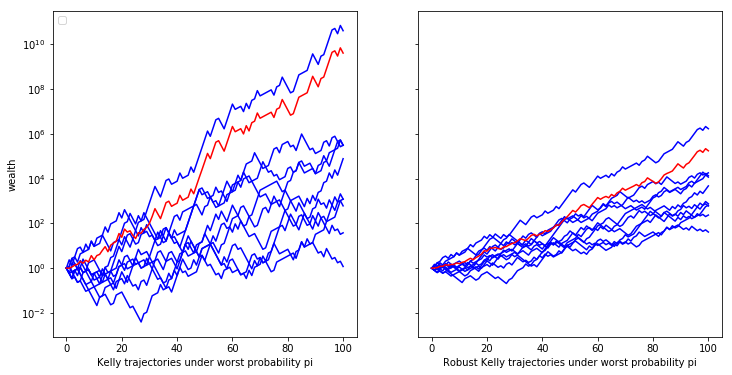
\includegraphics[width=1.\textwidth]{./Plot/Horse1}
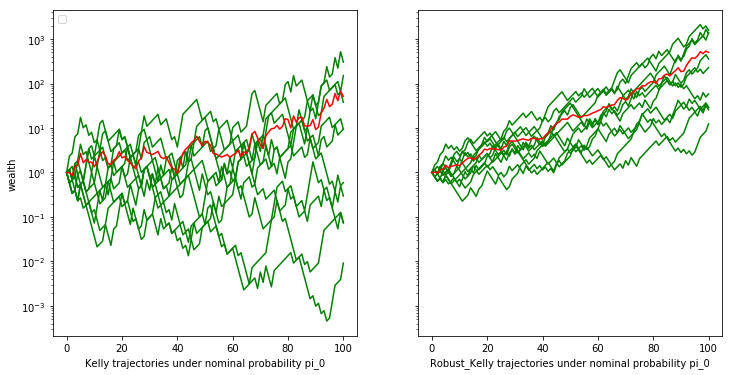
\includegraphics[width=1.\textwidth]{./Plot/Horse2}
\caption{Wealth trajectories comparison for Kelly optimal bet and DRKP under probability $\pi$ and nominal probability $\pi_0$. The red line are the mean of wealth over different realizations.}
\label{fig-time-domain-trajectories}
\end{figure}

% \paragraph{Financial investment}
% We consider a simple finite outcomes case
% with $20$ assets ($19$ risky assets and $1$ cash asset) and $K = 20$ possible outcomes, and we compare distributional robust bet with Kelly optimal bet in this case. 
% The problem data is generated as follows:
% the return matrix $R$ is given by table $1$; the worst probability is $\pi = (0.5, \frac{1}{2(K-1)}, \ldots, \frac{1}{2(K-1)})$, the uninformed  nominal probability is $\pi_0 = (1/K, \ldots, 1/K)$, assuming there is no information about $\pi$.
% \begin{table}
% \centering
% \begin{tabular}{c|c|c|c||c|c}
%       & Asset $1$ return & Asset $2$ return & Cash return &  $\pi$ &  $\pi_0$ \\
%       \hline
%       Case $1$ & 1.5 & 0.9 & 1 & 0.6 & 1/3 \\
%       Case $2$ & 0.5 & 1.1 & 1& 0.1 & 1/3\\
%       Case $3$ & 0.99 & 1.01 & 1& 0.3 & 1/3\\
%       \hline
% \end{tabular}
% \caption{Return matrix $R$ with the corresponding worst probability $\pi$ and nominal probability $\pi_0$.}
% \end{table} 

% Then for the distributional robust bet, we consider the  spherical probability set $\Pi = \{ \pi = \pi_0 + Z\delta, \quad  \|\delta\|_2 \leq 0.1, \quad \ones^T \pi = 1, \quad \pi \geq 0\}.$
% We generate samples from this returns distribution for Monte Carlo simulations.
% For any given allocation vector $b$, these simulations consist
% of $50$ trajectories of $w_t$ for $t=1, \ldots, 100$. From the plots of the simulation result \ref{fig-time-domain-trajectories}, we see that under the worst probability $\pi$, the DRKP does not hurt the performance of Kelly optimal bet too much; and under the nominal probability $\pi_0$, the DRKP performance better than simply holding cash, while the Kelly optimal bet leads to a very significant loss.

% \begin{figure} 
% \centering
% 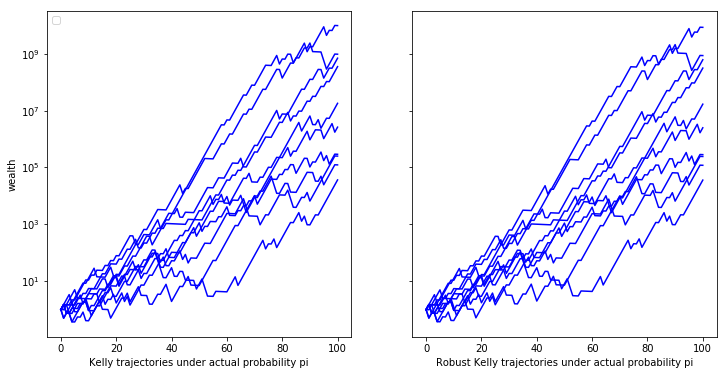
\includegraphics[width=1.\textwidth]{./Plot/correct_pi_3asset_3case_2}
% 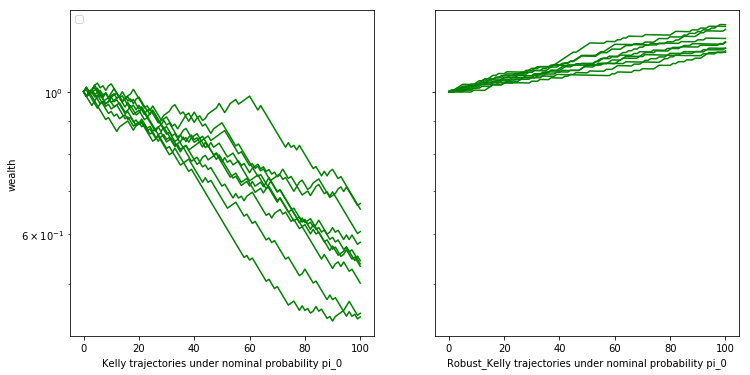
\includegraphics[width=1.02\textwidth]{./Plot/wrong_pi_3asset_3case_2}
% \caption{Wealth trajectories comparison for Kelly optimal bet and DRKP under worst probability $\pi$ and nominal probability $\pi_0$.}
% \label{fig-time-domain-trajectories}
% \end{figure}


\section{Appendix}
\paragraph{CVXPY code for examples}
\begin{itemize}
\item
For box constraint, 
$\{ \pi = \pi_0 + \delta, \quad -l\leq \delta\leq l, \quad \ones^T \pi = 1, \quad \pi \geq 0\}.$ 
The problem is
\BEQ
\begin{array}{ll}
\text{maximize}&  \left(\min_i   
(\log (R^T b)+  \mu)_i \right) 
-  \pi_0^T |\mu| - l^T \mu \\
\text{subject to} & b\in B,
\end{array}
\EEQ
with variables $b, \mu$.
It can be formulated and solved in CVXPY as 
\begin{verbatim}
pi_0 = Parameter(K,sign = 'positive')
L = Parameter(K,sign = 'positive')
b = Variable(n)
mu = Variable(K)
robust_growth_rate = 
min_entries(log(r.T*b) + mu )-pi_0.T*abs(mu )-L.T*mu 
constraints = [sum_entries(b) == 1, b >= 0] 
robust_Kelly= Problem(Maximize(robust_growth_rate), constraints)
robust_Kelly.solve() 
\end{verbatim}
Here \verb|r| is the matrix whose columns are the return 
vectors, \verb|pi_0| is the vector of probabilities $\pi_0$ and \verb|L| is $K$ dimensional box constraint $l$.
The second to last line forms the problem, and in the 
last line the problem is solved.  The robust optimal bet is written into
\verb|b.value|.
\item
For ellipsoid constraint under $p$-norm,
DRKP becomes
\BEQ 
\begin{array}{ll}\text{minimize}&  \|W (F -\mu 1)\|_q + \pi_0^T F\\
\text{subject to} &  b\in B, F\geq -\log (R^T b),
\end{array}
\EEQ
with variables $b, F, \mu$. 
It can be formulated and solved in CVXPY as 
\begin{verbatim}
pi_0 = Parameter(K,sign = 'positive')
w = Parameter(K,sign = 'positive')
b = Variable(n)
F = Variable(K)
mu = Variable(1)
neg_log_growth = -log(r.T*b)
robust_obj = pi_0.T*F+norm(mul_elemwise(w,F-mu*np.ones(K)),q)
constraints = [sum_entries(b) == 1, b >= 0, F>=neg_log_growth] 
robust_Kelly= Problem(Minimize(robust_obj), constraints)
robust_Kelly.solve() 
\end{verbatim}
Here \verb|pi_0| is again the vector of probabilities $\pi_0$, \verb|w| is the weight vector.
\end{itemize}




% \section{Remarks when probability set is independent of action}
% \paragraph{Convex concave game}
% In general, the distributional robust Kelly problem is a convex concave game. Explicitly, we can think of the  decision problem as a two-player zero-sum game between decision maker and nature. The decision maker act to place bets $b$ inside the actionable set $B$, and nature decides distribution of return $\pi$ inside the confidence set $\Pi$, and the game has a payoff function $G_\pi(b)$. Since the problem is convex to $\pi\in \Pi$, and concave to $b \in B$, it is a  convex concave game, and we are looking for a saddle-point.
% This problem can be efficiently solved using interior-point methods, as described in e.g. \cite{boyd2004convex}. 

% From general theory of convex concave game, when $\Pi$ is dependent of $b$, we know there are two related problems. 
% The first problem is when nature acts first, then decision maker acts to maximize the payoff. This is the robust Kelly gambling problem.
% \BEQ
% \label{robust-problem}
% \begin{array}{ll}
% \text{maximize}_{~b \in B} \quad \inf_{~\pi \in\Pi}  &\pi^T \log (R^T b).
% \end{array}
% \EEQ
% The second problem is when nature chooses $\pi$ first, then decision maker places bets $b$ to maximize the payoff. 
% \BEQ
% \label{dual problem}
% \begin{array}{ll}
%  \quad \text{minimize}_{~\pi \in\Pi} \quad \sup_{~b \in B}  &\pi^T \log (R^T b).
% \end{array}
% \EEQ
% This optimal value of second problem provide a lower-bound on the optimal value of the first problem. Furthermore,  using von Neumann's minimax theorem, since this is a convex-concave game with compact convex sets $\Pi,B$ and a continuous function $ G(\pi, b) = \pi^T \log (R^T b)$ that is convex-concave, we have that 
% \BEQ
% \label{robust-problem}
% \begin{array}{ll}
%  \text{maximize}_{~b \in B} \quad \inf_{~\pi \in\Pi}   \quad\pi^T \log (R^T b) 
% =  \text{minimize}_{~\pi \in\Pi} \quad \sup_{~b \in B} \quad  \pi^T \log (R^T b).
% \end{array}
% \EEQ
% \paragraph{Epigraph form}
% In general we can rewrite the problem in epigraph form, 
% \BEQ\label{ }
% \begin{array}{ll}
% \text{maximize}_{~b\in B } & t \\
% \text{subject to} 
% &  t-\pi^T \log (R^T b)\leq 0, \forall \pi \in\Pi .
% \end{array}
% \EEQ
% We can view this problem as a semi-infinite programming (SIP) problem, since we have an infinite number of constraints, parametrized by $\pi \in\Pi$. There is a massive literature for the solution of SIP problems, 
% % see
% we will not go into the details here.







\subsection*{Acknowledgments}
We thank Enzo Busseti 
for useful discussions.

% \bibliographystyle{unsrt}
\bibliographystyle{alpha}
\bibliography{robust_kelly}
\end{document}

